\chapter{Resultados}\label{cap_resultados}
\section{Imagem simulada}
A metodologia para a detecção de bordas baseadas em~\citet{gmbf}, \citet{gamf, nhfc} foi aplicada em uma imagem simulada particionada em duas classes. Essa imagem tem dimensão de $400\times400$ píxeis e foi gerada por duas amostras, obedecendo a distribuição Wishart. Na  classe da esquerda foi usada a matriz de covariâncias $\Sigma_{k_1}$, e na classe da direita a matriz de covariâncias $\Sigma_{k_2}$, respectivamente definidas por:
%%% ACF De onde vêm esses parâmetros?
%%% AAB citado
\begin{equation}\nonumber
\small
\Sigma_{k_1}= \left[
\begin{array}{lll}
0.042811            & 0.000072-0.003180\hat{\imath} & 0.010435+0.005022\hat{\imath}\\
0.000072+0.003180\hat{\imath}  & 0.035977           & 0.000784+0.004886\hat{\imath}\\
0.010435-0.005022\hat{\imath}  & 0.000784-0.004886\hat{\imath} & 0.066498
\end{array}
\right],
\end{equation}
\begin{equation}\nonumber
\small
 \Sigma_{k_2}= \left[
\begin{array}{lll}
0.014380            & 0.001333-0.000076\hat{\imath} & -0.000755+0.001570\hat{\imath}\\
0.001333+0.000076\hat{\imath}  & 0.002789           & -0.001044+0.001101\hat{\imath}\\
-0.000755-0.001570\hat{\imath} &-0.001044-0.001101\hat{\imath} & 0.015387
\end{array}
\right].
\end{equation}

As matrizes de covariância foram usadas para gerar resultados do artigo \citet{gamf}, os programas e dados usados no artigo estão disponíveis em \url{https://ctim.ulpgc.es/polsar/}.
  
As entradas das diagonais principais foram as intensidades usadas para gerar os canais $\mathbf{I_\text{hh}}$, $\mathbf{I_\text{hv}}$ e $\mathbf{I_\text{vv}}$ simulados. A decomposição de Pauli definida como sendo a combinação linear dos canais de intensidades, $(\mathbf{I_\text{hh}+I_{\text{vv}}}, \mathbf{I_\text{hh}-I_{\text{vv}}}, \mathbf{I_\text{hv}})$ foram usadas para compor a imagem. Veja a Figura~\ref{fig:simulada_gamf_dec_pauli}.  
\begin{figure}[hbt!]
	\centering
	\includegraphics[width=.5\linewidth]{phanton_gamf_dec_pauli_two_classes_crop}
	\caption{Decomposição de Pauli aplicada na imagem simulada}
\label{fig:simulada_gamf_dec_pauli}
\end{figure}

Nesta imagem simulada definimos a borda como a linha vertical que divide a imagem em duas classes. 
\subsection{Método estimativa de máxima verossimilhança aplicada a PDF Univariada Gamma}\label{sec:pdf_uni_gamma_apl_simulada}
O método MLE foi usado para detectar evidências de bordas em cada canal de intensidades, conforme descrito na seção~\ref{sec:eml_pdf_gamma}.


\begin{figure}[hbt!]
	\centering
     \subfloat[Canal simulado $\mathbf{I_\text{hh}}$]{%
       \includegraphics[width=0.5\linewidth]{graf_2d_gamf_2017_sigmahh_param_mu_L_linha_150}\label{fig:graf_2d_uni_gamma_param_mu_l:1a}}
     \subfloat[Canal simulado $\mathbf{I_\text{hv}}$]{%
       \includegraphics[width=0.5\linewidth]{graf_2d_gamf_2017_sigmahv_param_mu_L_linha_150}\label{fig:graf_2d_uni_gamma_param_mu_l:1b}}\\
     \subfloat[Canal simulado $\mathbf{I_\text{vv}}$]{%
       \includegraphics[width=0.5\linewidth]{graf_2d_gamf_2017_sigmavv_param_mu_L_linha_150}\label{fig:graf_2d_uni_gamma_param_mu_l:1c}}
     \caption{Funções de log-verossimilhanças reduzidas}
     \label{fig:graf_2d_uni_gamma_param_mu_l}
   \end{figure}	


As Figuras~\ref{fig:l_uni_gamma_param_mu_l}\subref{fig:l_uni_gamma_param_mu_l:1a},~\ref{fig:l_uni_gamma_param_mu_l}\subref{fig:l_uni_gamma_param_mu_l:1b},~\ref{fig:l_uni_gamma_param_mu_l}\subref{fig:l_uni_gamma_param_mu_l:1c} mostram os gráficos das funções de verossimi\-lhan\-ças totais~\eqref{eq:TotalLogLikelihood}, indicando as evidências de bordas para os canais de intensidades. A linha 150 da imagem simulada foi escolhida arbitrariamente, sendo que para cada extremidade foi definido a constante de folga igual a 14 píxeis. As constantes de folga foram definidas na seção \ref{sec:eml_pdf_gamma}. 

A característica comum dessas funções é não ser diferenciável, o que  dificulta o uso de métodos de otimização que calculam a derivada da função. O problema foi resolvido usando o método \textit{Simulated Annealing} generalizado \citep[GenSA][]{xgsh}, adequado para funções não diferenciáveis.
\begin{figure}[hbt!]
	\centering
     \subfloat[Canal simulado $\mathbf{I_\text{hh}}$]{%
       \includegraphics[width=0.34\linewidth]{grafico_l_gamf_2017_sigmahh_param_mu_L_linha_150}\label{fig:l_uni_gamma_param_mu_l:1a}}
     \subfloat[Canal simulado $\mathbf{I_\text{hv}}$]{%
       \includegraphics[width=0.34\linewidth]{grafico_l_gamf_2017_sigmahv_param_mu_L_linha_150}\label{fig:l_uni_gamma_param_mu_l:1b}}
     \subfloat[Canal simulado $\mathbf{I_\text{vv}}$]{%
       \includegraphics[width=0.34\linewidth]{grafico_l_gamf_2017_sigmavv_param_mu_L_linha_150}\label{fig:l_uni_gamma_param_mu_l:1c}}
     \caption{Funções de verossimilhanças totais para cada canal simulado}
     \label{fig:l_uni_gamma_param_mu_l}
   \end{figure}	
 
%<<<<<<< Updated upstream
%Assim, para cada linha dos canais de intensidades da imagem simulada. As evidências de bordas detectadas podem ser %visualizadas na figura \ref{evidencias_hh_hv_vv:a}.
%=======
As evidências de bordas detectadas em cada canal simulado hh, hv e vv podem ser visualizadas, respectivamente, nas  Figuras \ref{evidencias_hh_hv_vv_uni_gamma_gamf_mu_L:a}, \ref{evidencias_hh_hv_vv_uni_gamma_gamf_mu_L:b}, e \ref{evidencias_hh_hv_vv_uni_gamma_gamf_mu_L:c}.
%%% ACF Recorte *todas* as figuras PDF da tese. Veja como fica ruim com a borda que você deixou
%>>>>>>> Stashed changes
 \begin{figure}[htb!]
     \centering
     \subfloat[Evidências no canal $\mathbf{I_\text{hh}}$]{%
       \includegraphics[width=0.33\linewidth]{im_sim_gamf_hh_evid_param_mu_L_14_pixel_crop}
      \label{evidencias_hh_hv_vv_uni_gamma_gamf_mu_L:a}    
     }
     \subfloat[Evidências no canal $\mathbf{I_\text{hv}}$]{%
       \includegraphics[width=0.33\linewidth]{im_sim_gamf_hv_evid_param_mu_L_14_pixel_crop} \label{evidencias_hh_hv_vv_uni_gamma_gamf_mu_L:b}
     }
     \subfloat[Evidências no canal $\mathbf{I_\text{vv}}$]{%
       \includegraphics[width=0.33\linewidth]{im_sim_gamf_vv_evid_param_mu_L_14_pixel_crop} \label{evidencias_hh_hv_vv_uni_gamma_gamf_mu_L:c}
     }
    \caption{Evidências de bordas para os canais de intensidades.}
     \label{evidencias_hh_hv_vv_uni_gamma_gamf_mu_L} 
   \end{figure}
%
\subsection{Métricas para as evidências de bordas nas imagens simuladas}\label{sec:erro_evid_simulado}
%%% ACF O texto está confuso: é "erro de probabilidade de detecção"?. Reescreva
%%% Realizado
O erro de detecção, descrito \citet{fbgm}, é calculado com o seguinte procedimento:
\begin{itemize}
\item Em cada radial (linha) definida na imagem calcular a menor distância euclidiana entre a borda detectada e o pixel de referência \textit{Ground Reference} (GR). Se em uma mesma radial detectamos vários píxeis, calculamos todas as distâncias e armazenamos a menor.
\item Cada erro encontrado é comparado a uma constante definida neste trabalho como sendo $k_s=10$. Assim construímos o vetor de frequência $H(k)$, com $\{k=1,\dots,k_s\}$ , definindo o número de replicações para qual o erro é menor que a constante definida. 
\item  A estimativa de probabilidade é encontrada por $f(k)={H(k)}/{n_r}$, onde  $n_r$ é o número de radiais.
\end{itemize} 
 
%<<<<<<< Updated upstream
A Figura \ref{metrica_sim_port} mostra o gráfico do erro de detecção para cada canal simulado.
%=======
%A figura (\ref{metrica_sim_port}) mostra o gráfico do erro de probabilidades de detecção para cada canal simulado.
%%% ACF Precisa padronizar o estilo de todos os gráficos. Sugiro usar o estilo desta figura.
%>>>>>>> Stashed changes
\begin{figure}[hbt!]
	\centering
	\includegraphics[width=.50\linewidth]{metricas_simuladas_port}%
	\caption{Métricas para a detecção em imagem simulada}
\label{metrica_sim_port}
\end{figure}

%<<<<<<< Updated upstream
O gráfico mostra acurado desempenho do algoritmo no canal hv. Nos canais hh e vv o desempenho é inferior em relação ao canal hv. O desempenho acurado do método MLE para a detecção de borda no canal hv já poderia ser inferido pela inspeção visual da Figura \ref{evidencias_hh_hv_vv_uni_gamma_gamf_mu_L}. 
%=======
%O gráfico mostra acurado desempenho do algoritmo no canal hv. Nos canais hh e vv o desempenho é inferior em relação ao canal hv, fato que já poderia ser inferido pela inspeção visual da figura~\eqref{evidencias_hh_hv_vv_uni_gamma_gamf_mu_L:a}. 
%%% ACF Por que poderia ser inferido?
%%% Realizado
%
%>>>>>>> Stashed changes
\subsection{Fusão de evidências de bordas para os canais de intensidades}
Os resultados dos métodos para a fusão de evidências de bordas detectadas nos canais simulados são mostrados nas Figuras~\ref{sim_fusion_met}\subref{sim_fusion_met:a}, \subref{sim_fusion_met:b}, \subref{sim_fusion_met:c}, \subref{sim_fusion_met:d}, \subref{sim_fusion_met:e}, e~\subref{sim_fusion_met:f}.  

%%% ACF Veja como as bordas deixam a figura ruim
%%% AAB Realizado
\begin{figure}[htb!]
	\centering
     \subfloat[Fusão por média\label{sim_fusion_met:a}]{%
       \includegraphics[width=0.4\linewidth]{sim_fus_media_param_L_mu_14_pixel_crop}
     }
     \subfloat[Fusão DWT\label{sim_fusion_met:b}]{%
       \includegraphics[width=0.4\linewidth]{sim_fus_dwt_param_L_mu_14_pixel_crop}
     }\\
     \subfloat[Fusão PCA \label{sim_fusion_met:c}]{%
       %\includegraphics[width=0.2\textwidth]{example-image-a}
       \includegraphics[width=0.4\linewidth]{sim_fus_pca_param_L_mu_14_pixel_crop}       
     }
     \subfloat[Fusão E-ROC\label{sim_fusion_met:d}]{%
       \includegraphics[width=0.4\linewidth]{sim_fus_roc_param_L_mu_14_pixel_crop}
     }\\
     
     \subfloat[Fusão MR-SWT \label{sim_fusion_met:e}]{%
       \includegraphics[width=0.4\linewidth]{sim_fus_swt_param_L_mu_14_pixel_crop}
     }
     \subfloat[Fusão MR-SVD\label{sim_fusion_met:f}]{%
       \includegraphics[width=0.4\linewidth]{sim_fus_svd_param_L_mu_14_pixel_crop}
     }
     \caption{Resultados da aplicação dos seis métodos de fusão}
     \label{sim_fusion_met}
\end{figure}

A inspeção visual das figuras fornece elementos para as seguintes conclusões:
\begin{itemize}
\item O método de fusão PCA e a fusão por média obtém o mesmo resultado pixel a pixel, a vantagem do método de fusão PCA está na ponderação dos canais que contribuem na fusão, fornecendo subsídios para o descarte ou a valorização de um devido canal;
\item Os métodos de fusão baseados nas transformadas wavelets mapeiam de forma acurada as bordas, porém ocorre a geração de \textit{outliers}.
\item O método E-ROC mostra um bom desempenho na fusão de evidências de bordas, principalmente com relação a geração de \text{outliers}, lembrando que é o único método que foram aplicados limiares.
\item O método de fusão baseado em decomposição de valores singulares apresenta bom desempenho na fusão e gera pouco \textit{outliers}.
\end{itemize}

A Figura~\ref{metrica_sim_fus_3_canais_port} mostra o gráfico do erro de detecção para os métodos de fusão de evidências de bordas.
\begin{figure}[hbt!]
	\centering
	\includegraphics[width=.50\linewidth]{metricas_simuladas_fus_3_canais_port}%
	\caption{Métricas para a fusão de evidências de bordas}
\label{metrica_sim_fus_3_canais_port}
\end{figure}

A imagem simulada de duas classes produz regiões homogêneas, as bordas são bem definidas, por isso os métodos de fusão trabalham com grande precisão e geram sobreposições dos erros de detecção no gráfico, como pode ser visto na Figura \ref{metrica_sim_fus_3_canais_port}.   

Comparando os gráficos das Figuras \ref{metrica_sim_port}  e \ref{metrica_sim_fus_3_canais_port} podemos notar que os métodos de fusão melhoram o desempenho em detectar bordas precisas com relação aos métodos de detectar as evidências de bordas para cada canal. Podemos confirmar assim o melhor desempenho dos métodos de fusão.

O método de fusão para a curva ROC mostra um desempenho abaixo dos outros métodos em relação a probabilidade de indicar se o pixel é borda ou não. Esse método tem potencial para melhorar seu desempenho a medida que inserirmos outros canais para a detecção de evidências de bordas. 

 Os resultados obtidos com a aplicação desses métodos validaram os algoritmos usados, essa etapa foi crucial para o desenvolvimento deste trabalho, viabilizando a realização dos testes em imagens adquiridas de sensores PolSAR.
\section{Imagens adquiridas por sensores PolSAR}
Os métodos apresentados neste trabalho foram executados com um computador Intel\copyright\ Core i7-9750HQ CPU 
\SI{2.6}{\giga\hertz} \SI{16}{\giga\byte}. O erro foi medido com o mesmo método aplicado na imagem simulada.
\subsection{Imagem de Flevoland}
%<<<<<<< Updated upstream
%A imagem da região de Flevoland com dimensão $750\times 1024$ pixeis é uma imagem PolSAR capturada pelo sensor aerotransportado AIRSAR com banda-L. A imagem tem 4 visadas, 9 canais, e uma resolução de aproximadamente 12,10 metros na direção azimutal e 6,6 metros na direção lateral do sensor. A decomposição de Pauli da imagem capturada no sensor é mostrada na figura~\ref{flevoland_4_look}. 
%=======
A imagem da região de Flevoland com dimensão $750\times 1024$ píxeis é uma imagem PolSAR capturada pelo sensor aerotransportado AIRSAR com banda-L. A imagem tem 4 visadas, 9 canais, e uma resolução de aproximadamente \SI{12,10}{\meter} na direção azimutal e \SI{6,6}{\meter} na direção lateral do sensor. A decomposição de Pauli da imagem capturada no sensor é mostrada na Figura \ref{flevoland_4_look}. 
%>>>>>>> Stashed changes
\begin{figure}[htb!]
	\centering
	\includegraphics[width=.40\linewidth]{flevoland_4_look}%
	\caption{Imagem da região de Flevoland}
\label{flevoland_4_look}
\end{figure}

%A figura~\eqref{flevoland_4_look_radial} mostra as radiais usadas para extrair as informações da imagem de Flevoland. 
%\begin{figure}[hbt]
%	\centering
%	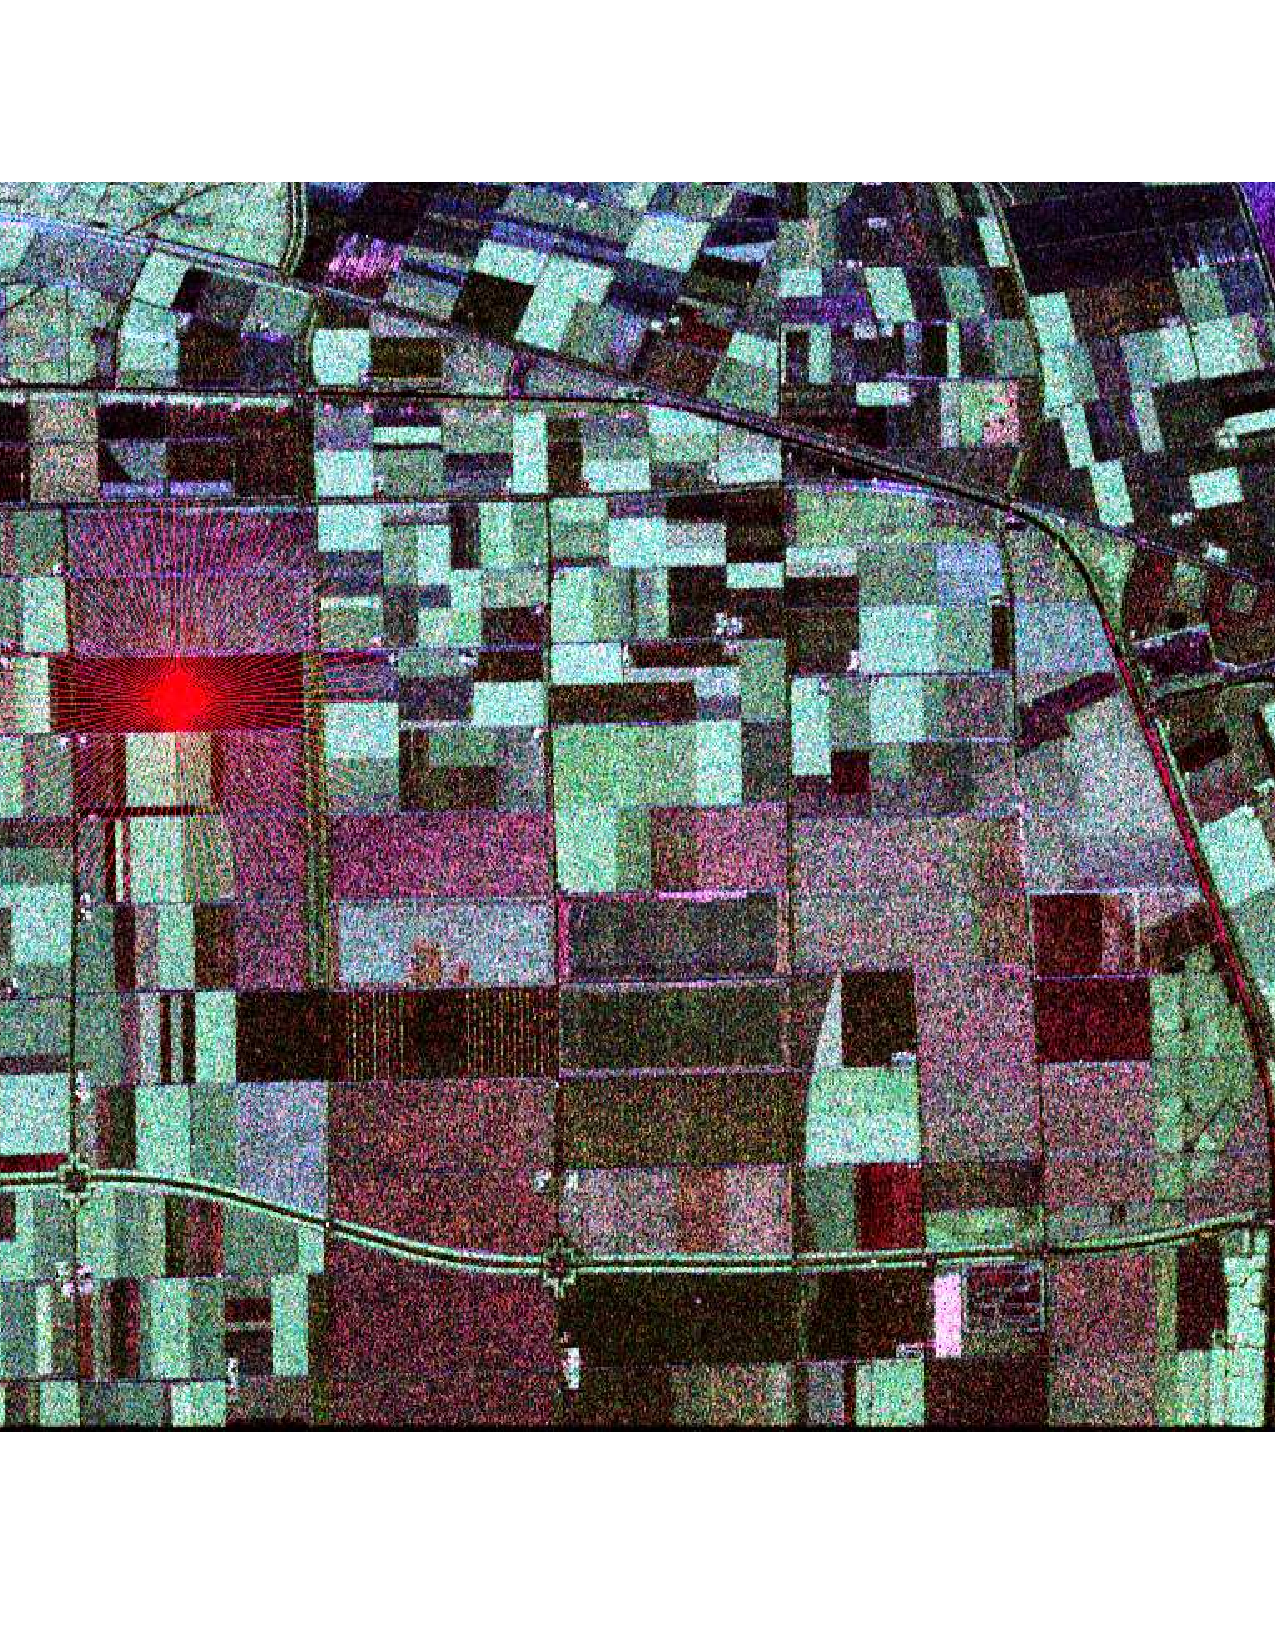
\includegraphics[width=.40\linewidth]{flevoland_radial_4_look}%
%	\caption{Imagem da região de Flevoland com radiais}
%\label{flevoland_4_look_radial}
%\end{figure}
%\clearpage

\subsubsection{FLEV-ROI-I}
%<<<<<<< Updated upstream
%Os métodos desenvolvidos neste trabalho foram aplicados na região de interesse destacada na imagem. Detalhes da região de interesse, e das radiais usadas para extrair informações podem ser vista na figura~\ref{roi_gt}\subref{flevoland_radial_4_look_crop}. A figura~\ref{roi_gt}\subref{gt_flevoland_crop} mostra em pixeis vermelhos, as bordas que são usadas como referência, conhecida por imagem \textit{Ground Truth} (GT). Região de interesse é denominada FLEV-ROI-I.  
%=======
Os métodos desenvolvidos neste trabalho foram aplicados na região de interesse destacada na imagem. Detalhes da região de interesse, e das radiais usadas para extrair informações podem ser vista na Figura~\ref{roi_gt}\subref{flevoland_radial_4_look_crop}. A Figura~\ref{roi_gt}\subref{gt_flevoland_crop} mostra em píxeis vermelhos, as bordas que são usadas como referência, conhecida por imagem \textit{Ground Reference} (GR). 
A região de interesse é denominada FLEV-ROI-I.  

%>>>>>>> Stashed changes
\begin{figure}[hbt!]
   \centering
     \subfloat[Imagem, ROI, e radiais. \label{flevoland_radial_4_look_crop}]{%  
       \includegraphics[width=0.229\textwidth]{flevoland_radial_4_look_black_crop}}
     \subfloat[\textit{Ground Reference}\label{gt_flevoland_crop}]{%
       \includegraphics[width=0.216\textwidth]{gt_flevoland_crop}
     }
    \caption{Região de interesse da imagem Flevoland (FLEV-ROI-I), e \textit{Ground Reference} de referência}
    \label{roi_gt}
\end{figure}

As Figuras~\ref{evidencias_hh_hv_vv}\subref{evidencias_hh_hv_vv:a}, \ref{evidencias_hh_hv_vv}\subref{evidencias_hh_hv_vv:b}, e~\ref{evidencias_hh_hv_vv}\subref{evidencias_hh_hv_vv:c} mostram, respectivamente, as evidências de bordas nos canais~$\text{hh}$, $\text{hv}$,~e~$\text{vv}$, obtidas pelo método MLE. Para a FLEV-ROI-I foi estabelecido 100 radiais com comprimento de 120 píxeis, onde foi constatado uma forte oscilação da função de máxima verossimilhança total nos píxeis dos extremos das radiais,  para evitar a oscilação nesta região foi definida uma folga com 14 píxeis. Esse valor foi escolhido empiricamente e pode variar de acordo com a região de interesse da imagem, o canal, o sensor e a imagem. Na FLEV-ROI-I os 14 píxeis, escolhidos para cada extremidade, foram suficientes para contornar o problema da oscilação.

%%% ACF Parágrafo confuso. Escreva de forma mais direta, quiçá dividindo-o em duas frases
Os parâmetros para as funções de máxima verossimilhança reduzidas são estimados pelo método BFGS usando o programa MaxLik. Estes parâmetros estimados são aplicados nas funções de máxima verossimilhança total com o objetivo de  encontramos o seu valor máximo e o seu argumento. O método GenSA foi usado para realizar este processo de maximização, obtendo as evidências de bordas com precisão.  
\begin{figure}[hbt!]
	\centering
    \subfloat[Canal $\text{hh}$ \label{evidencias_hh_hv_vv:a}]{%
    	\includegraphics[width=0.32\linewidth]{flevoland_hh_evid_param_L_mu_14_pixel_crop}
     	}
    \subfloat[Canal $\text{hv}$ \label{evidencias_hh_hv_vv:b}]{%
       	\includegraphics[width=0.32\linewidth]{flevoland_hv_evid_param_L_mu_14_pixel_crop}
     	}
    \subfloat[Canal $\text{vv}$ \label{evidencias_hh_hv_vv:c}]{%
       	\includegraphics[width=0.32\linewidth]{flevoland_vv_evid_param_L_mu_14_pixel_crop}
     	}
    \caption{Evidências de bordas para os três canais de intensidades na FLEV-ROI-I}
    \label{evidencias_hh_hv_vv} 
\end{figure}

A inspeção visual destas figuras mostra a melhor acurácia dos métodos no canal hv, e presença de \textit{outliers} no canal vv.

A Figura~\ref{metricas_evid_3_canais_flevoland_port} mostra o gráfico do erro de detecção para os métodos de fusão de evidências de bordas na região FLEV-ROI-I.
\begin{figure}[hbt!]
	\centering
	\includegraphics[width=.50\linewidth]{metricas_evid_3_canais_flevoland_port}%
	\caption{Métricas para a fusão de evidências de bordas na região FLEV-ROI-I}
\label{metricas_evid_3_canais_flevoland_port}
\end{figure}
O canal hv apresenta o melhor desempenho, comprovando a inspeção visual.

Figuras~\ref{fusion_met}\subref{fusion_met:a}, \subref{fusion_met:b}, \subref{fusion_met:c}, \subref{fusion_met:d}, \subref{fusion_met:e}, e~\subref{fusion_met:f} mostram os resultados numéricos para os métodos propostos de fusão de evidência de bordas.
\clearpage 
\begin{figure}[hbt!]
	\centering
     \subfloat[Fusão por média\label{fusion_met:a}]{%
       \includegraphics[width=0.3\linewidth]{flevoland_fus_media_param_L_mu_14_pixel_crop}
     }
     \subfloat[Fusão DWT\label{fusion_met:b}]{%
       \includegraphics[width=0.3\linewidth]{flevoland_fus_dwt_param_L_mu_14_pixel_crop}
     }\\
     \subfloat[Fusão PCA \label{fusion_met:c}]{%
       %\includegraphics[width=0.2\textwidth]{example-image-a}
       \includegraphics[width=0.3\linewidth]{flevoland_fus_pca_param_L_mu_14_pixel_crop}       
     }
     \subfloat[Fusão E-ROC\label{fusion_met:d}]{%
       \includegraphics[width=0.3\linewidth]{flevoland_fus_roc_param_L_mu_14_pixel_crop}
     }\\
     \subfloat[Fusão MR-SWT \label{fusion_met:e}]{%
       \includegraphics[width=0.3\linewidth]{flevoland_fus_swt_param_L_mu_14_pixel_crop}
     }
     \subfloat[Fusão MR-SVD\label{fusion_met:f}]{%
       \includegraphics[width=0.3\linewidth]{flevoland_fus_svd_param_L_mu_14_pixel_crop}
     }
     \caption{Métodos de fusão para a região FLEV-ROI-I}
     \label{fusion_met}
\end{figure}

A Figura~\ref{probability_edge_detc_flev_roi_i} mostra o erro dos métodos de fusão para a FLEV-ROI-I com o número de radiais igual a 100.
\begin{figure}[hbt!]
\centering
	\includegraphics[width=.5\linewidth]{metricas_6_fusao_flevoland_port}
	\caption{Métricas para a fusão de evidências de bordas na região FLEV-ROI-I}
\label{probability_edge_detc_flev_roi_i}
\end{figure}

Os métodos de fusão por média e fusão PCA produzem resultados similares, veja Figura~\ref{probability_edge_detc_flev_roi_i}. A vantagem do método PCA está em realizar a média ponderada das evidências de bordas nos diferentes canais, possibilitando a quantificação da importância de cada canal no processo de fusão.

O MR-SVD produz uma considerável vantagem em descartar \text{outliers}, porém o tempo de processamento é maior em comparação com os demais métodos.

O método usando a estatística ROC produz bordas acuradas, com poucos \text{outliers}, porém de forma esparsa. Acreditamos que este método tem potencial na medida em que mais canais forem considerados, ou ao serem aplicadas outras funções de densidades de probabilidades para obter evidências de bordas. 

Os métodos baseados em \textit{wavelets} produzem densas bordas, mesmo mostrando serem melhores em probabilidade de detectar bordas, os métodos produzem \text{outliers}. Destacamos que a detecção pode ser melhorada com o uso de pós-processamento \citep{fbgm}, podendo ser aplicado em todos os métodos, inclusive em cada canal onde as evidências forem detectadas. 

Os dados apresentados na primeira linha da Tabela~\ref{metrica_de_tempo_3_canais} indicam o tempo de processamento para cada método de fusão. Na segunda linha contém os tempos de cada métodos relativo com a fusão por média, por ser o mais rápido. 
\begin{table}[hbt]
\small
	\centering
	\caption{Tempo de processamento para os métodos de fusão}\label{metrica_de_tempo_3_canais}
	\begin{tabular}{@{}lrrrrrr@{}} \toprule
		Método        & Média     &   PCA      &  MR-DWT  & MR-SWT    &  ROC  &  MR-SVD \\ \midrule
		Tempo (s)     & 0.00909075&0.01865585  & 0.1093859& 0.18789595&  0.4574247 &  1.1683798  \\
		Time Rel.     & 1.00      & 2.05       & 12.03    & 20.66     &   50.31     & 128.52  \\ \bottomrule
	\end{tabular}
\end{table}

%% Teste com a região II Flevoland
%%%  25 radials lenght 120 - com folga 14
\clearpage
\subsubsection{FLEV-ROI-II}
Uma segunda região na imagem de Flevoland foi selecionada para os testes a qual denominamos de região de interesse FLEV-ROI-II. A imagem com as radiais é mostrada na Figura~\ref{roi_gt_roi_ii}\subref{flevoland_radial_25_crop_roi_ii}. A Figura~\ref{roi_gt_roi_ii}\subref{gt_flevoland_crop_roi_ii} mostra as bordas em píxeis vermelhos usadas de referência a qual chamaremos de \textit{Ground Reference} (GR).
\begin{figure}[hbt!]
   \centering
     \subfloat[Imagem, ROI, e radiais. \label{flevoland_radial_25_crop_roi_ii}]{%  
       \includegraphics[width=0.216\textwidth]{flevoland_r3_radial_crop}}
     \subfloat[\textit{Ground Reference}\label{gt_flevoland_crop_roi_ii}]{%
       \includegraphics[width=0.216\textwidth]{gt_flevoland_r3_crop}
     }
     \caption{Região de interesse da imagem Flevoland (FLEV-ROI-II), e \textit{Ground Reference} de referência}
    \label{roi_gt_roi_ii}
\end{figure}
   
As Figuras~\ref{evidencias_flev_roi_ii_25_pixel_hh_hv_vv:a}\subref{evidencias_flev_roi_ii_25_pixel_hh_hv_vv:a} \ref{evidencias_flev_roi_ii_25_pixel_hh_hv_vv}\subref{evidencias_flev_roi_ii_25_pixel_hh_hv_vv:b} e~\ref{evidencias_flev_roi_ii_25_pixel_hh_hv_vv}\subref{evidencias_flev_roi_ii_25_pixel_hh_hv_vv:c} mostram, respectivamente, as evidências de bordas nos canais hh, hv e vv, obtidas pelo método MLE. Para a FLEV-ROI-II foi estabelecido 25 radiais com comprimento de 120 píxeis.  Nas extremidades em cada radial foi utilizado uma folga de 25 píxeis, pois foi constatado forte oscilação da função de máxima verossimilhança total. Esse valor foi escolhido empiricamente e pode variar de acordo com a região, o canal e a imagem. 
   \begin{figure}[hbt!]
	\centering
     \subfloat[Canal $\text{hh}$ \label{evidencias_flev_roi_ii_25_pixel_hh_hv_vv:a}]{%
       \includegraphics[width=0.32\linewidth]{evid_real_flev_hh_param_L_mu_25_pixel_r3_crop}
     }
     \subfloat[Canal $\text{hv}$ \label{evidencias_flev_roi_ii_25_pixel_hh_hv_vv:b}]{%
       \includegraphics[width=0.32\linewidth]{evid_real_flev_hv_param_L_mu_25_pixel_r3_crop}
     }
     \subfloat[Canal $\text{vv}$ \label{evidencias_flev_roi_ii_25_pixel_hh_hv_vv:c}]{%
       \includegraphics[width=0.32\linewidth]{evid_real_flev_vv_param_L_mu_25_pixel_r3_crop}
     }
          \caption{Evidências de bordas para os três canais de intensidades para FLEV-ROI-II na imagem de Flevoland com folga de 25 píxeis}
     \label{evidencias_flev_roi_ii_25_pixel_hh_hv_vv} 
   \end{figure}
   
A Figura~\ref{metricas_evid_3_canais_flevoland_port_r2} mostra o gráfico do erro de detecção para os métodos de fusão de evidências de bordas na região FLEV-ROI-II. Ao observá-la podemos constatar que o canal hv apresenta maior probabilidade de detectar bordas acuradas, confirmando a inspeção visual.   
Na FLEV-ROI-II, a escolha de 25 píxeis, em cada extremidade, foi suficientes para contornar o problema da oscilação. 

\begin{figure}[hbt!]
	\centering
	\includegraphics[width=.50\linewidth]{metricas_evid_3_canais_flev_roi_2_port}%
	\caption{Métricas para a detecção de evidências de bordas na região FLEV-ROI-II}
\label{metricas_evid_3_canais_flevoland_port_r2}
\end{figure}

Os resultados das aplicações dos métodos de fusão estudados estão expostos nas Figuras~\ref{fusion_flev_roi_ii_25_pixel_met}\subref{fusion_flev_roi_ii_25_pixel_met:a}, \subref{fusion_flev_roi_ii_25_pixel_met:b}, \subref{fusion_flev_roi_ii_25_pixel_met:c}, \subref{fusion_flev_roi_ii_25_pixel_met:d}, \subref{fusion_flev_roi_ii_25_pixel_met:e}, e~\subref{fusion_flev_roi_ii_25_pixel_met:f}.

\begin{figure}[hbt!]
	\centering
     \subfloat[Fusão por média\label{fusion_flev_roi_ii_25_pixel_met:a}]{%
       \includegraphics[width=0.32\linewidth]{flev_r3_fus_media_param_L_mu_25_pixel_crop}
     }
     \subfloat[Fusão DWT\label{fusion_flev_roi_ii_25_pixel_met:b}]{%
       \includegraphics[width=0.32\linewidth]{flev_r3_fus_dwt_param_L_mu_25_pixel_crop}
     }\\
     \subfloat[Fusão PCA \label{fusion_flev_roi_ii_25_pixel_met:c}]{%
       \includegraphics[width=0.32\linewidth]{flev_r3_fus_pca_param_L_mu_25_pixel_crop}       
     }
     \subfloat[Fusão E-ROC\label{fusion_flev_roi_ii_25_pixel_met:d}]{%
       \includegraphics[width=0.32\linewidth]{flev_r3_fus_roc_param_L_mu_25_pixel_crop}
     }\\
     \subfloat[Fusão MR-SWT \label{fusion_flev_roi_ii_25_pixel_met:e}]{%
       \includegraphics[width=0.32\linewidth]{flev_r3_fus_swt_param_L_mu_25_pixel_crop}
     }
     \subfloat[Fusão MR-SVD \label{fusion_flev_roi_ii_25_pixel_met:f}]{%
       \includegraphics[width=0.32\linewidth]{flev_r3_fus_svd_param_L_mu_25_pixel_crop}
     }
     \caption{Resultados das aplicações dos métodos de fusão para a FLEV-ROI-II com 25 píxeis de folga}
     \label{fusion_flev_roi_ii_25_pixel_met}
\end{figure}

A Figura~\ref{probability_edge_detc_flev_roi_ii} mostra o erro de detecção dos métodos de fusão para a FLEV-ROI-II.

\begin{figure}[hbt!]
\centering
	\includegraphics[width=.5\linewidth]{metricas_6_fusao_flevoland_r3_port}
    \caption{Métricas para a fusão de evidências de bordas na região FLEV-ROI-II}	 
\label{probability_edge_detc_flev_roi_ii}
\end{figure}

Os resultados dos métodos de fusão não tiveram mudanças significativas quando as fusões foram aplicadas na região FLEV-ROI-I ou na região FLEV-ROI-II.  

\subsubsection{Imagem de São Francisco}
A imagem da baía de São Francisco de dimensão $450\times 600$ píxeis é uma imagem PolSAR capturada pelo sensor aerotranportado AIRSAR com banda-L. A imagem tem 4 visadas, 9 canais, e uma resolução de aproximadamente \SI[product-units = brackets-power]{10 x 10}{\metre}. A decomposição de Pauli da imagem capturada no sensor é exposta na Figura~\eqref{san_francisco}.
%%% ACF Informar a resolução espacial
%%% AAB Realizado

\begin{figure}[hbt!]
	\centering
	\includegraphics[width=.5\linewidth]{san_francisco_2020}%
	\caption{Imagem da baía de São Francisco}
\label{san_francisco}
\end{figure}
%% Teste com a região I San Francisco
%%% radial lenght 120 - com folga 25

Na Figura~\ref{roi_san_fran_gt}\subref{san_francisco_radial_25} é destacada a região de interesse (SF-ROI) com 25 radiais. Em cada radial foram extraídos os dados para obter as informações sobre as localizações das evidências de bordas. A Figura~\ref{roi_san_fran_gt}\subref{gt_san_fran_r1_crop} mostra a imagem \textit{Ground Reference} (GR) que foi gerada para validar os resultados.  
\begin{figure}[hbt!]
   \centering
     \subfloat[Imagem, ROI e radiais. \label{san_francisco_radial_25}]{%  
       \includegraphics[width=0.216\textwidth]{san_francisco_radial_25_crop}}
     \subfloat[\textit{Ground Reference}\label{gt_san_fran_r1_crop}]{%
       \includegraphics[width=0.216\textwidth]{gt_san_fran_r1_crop}
     }%
     \caption{Decomposição de Pauli para imagem de São Francisco, e a \textit{Ground Reference} - GR}
    \label{roi_san_fran_gt}
\end{figure}

As Figuras.~\ref{evidencias_sf_hh_hv_vv}\subref{evidencias_sf_hh_hv_vv:a}, \ref{evidencias_sf_hh_hv_vv}\subref{evidencias_sf_hh_hv_vv:b}, e~\ref{evidencias_sf_hh_hv_vv}\subref{evidencias_sf_hh_hv_vv:c} mostram, respectivamente, as evidências de bordas nos canais hh, hv e vv, obtidos pelo método MLE. Para a SF-ROI foram estabelecidos 25 radiais com comprimento de 120 píxeis. Nas extremidades de cada radial foi estabelecido uma folga de 25 píxeis, pois foi constatado forte oscilação da função de máxima verossimilhança total. Esse valor foi escolhido empiricamente e pode variar de acordo com a região, o canal e a imagem. 
Na SF-ROI os 25 píxeis escolhidos em cada extremidade foram suficientes para contornar o problema  da oscilação.
\begin{figure}[htb!]
	\centering
     \subfloat[Canal $\text{hh}$ \label{evidencias_sf_hh_hv_vv:a}]{%
       \includegraphics[width=0.32\linewidth]{evid_real_sf_1_param_L_mu_25_pixel_r1_crop}
     }
     \subfloat[Canal $\text{hv}$ \label{evidencias_sf_hh_hv_vv:b}]{%
       \includegraphics[width=0.32\linewidth]{evid_real_sf_2_param_L_mu_25_pixel_r1_crop}
     }
     \subfloat[Canal $\text{vv}$ \label{evidencias_sf_hh_hv_vv:c}]{%
       \includegraphics[width=0.333\linewidth]{evid_real_sf_3_param_L_mu_25_pixel_r1_crop}
     }
     \caption{Evidências de bordas para os canais de intensidades na imagem de são Francisco}
     \label{evidencias_sf_hh_hv_vv} 
\end{figure}
A inspeção visual mostra bordas com melhor acurácia no canal hh.

A Figura~\ref{metricas_evid_3_canais_sf_port} mostra o gráfico do erro de detecção para os métodos de fusão de evidências de bordas na região SF-ROI.
\begin{figure}[hbt!]
	\centering
	\includegraphics[width=.50\linewidth]{metricas_evid_3_canais_sf_port}%
	\caption{Métricas para a fusão de evidências de bordas na região SF-ROI}
\label{metricas_evid_3_canais_sf_port}
\end{figure}
O canal hh apresenta o melhor desempenho comprovando a inspeção visual.

Nas Figuras~\ref{fusion_sf_met}\subref{fusion_sf_met:a}, \subref{fusion_sf_met:b}, \subref{fusion_sf_met:c}, \subref{fusion_sf_met:d}, \subref{fusion_sf_met:e}, e~\subref{fusion_sf_met:f} são apresentados os resultados numéricos obtidos com a aplicação dos métodos de fusão das evidência de bordas propostos neste trabalho. 
\begin{figure}[htb!]
	\centering
     \subfloat[Fusão por média\label{fusion_sf_met:a}]{%
       \includegraphics[width=0.3\linewidth]{sf_fus_media_param_L_mu_25_pixel_crop}
     }
     \subfloat[Fusão DWT\label{fusion_sf_met:b}]{%
       \includegraphics[width=0.3\linewidth]{sf_fus_dwt_param_L_mu_25_pixel_crop}
     }\\
     \subfloat[Fusão PCA\label{fusion_sf_met:c}]{%
       \includegraphics[width=0.3\linewidth]{sf_fus_pca_param_L_mu_25_pixel_crop}       
     }
     \subfloat[Fusão ROC\label{fusion_sf_met:d}]{%
       \includegraphics[width=0.3\linewidth]{sf_fus_roc_param_L_mu_25_pixel_crop}
     }\\
     \subfloat[Fusão MR-SWT\label{fusion_sf_met:e}]{%
       \includegraphics[width=0.3\linewidth]{sf_fus_swt_param_L_mu_25_pixel_crop}
     }
     \subfloat[Fusão MR-SVD\label{fusion_sf_met:f}]{%
       \includegraphics[width=0.3\linewidth]{sf_fus_svd_param_L_mu_25_pixel_crop}
     }
     \caption{Resultado da aplicação dos método de fusão para a SF-ROI}
     \label{fusion_sf_met}
\end{figure}

A Figura~\ref{probability_edge_detc_sf_roi_i} mostra o erro para SF-ROI com o número de radiais igual a 25.
\begin{figure}[hbt!]
\centering
	\includegraphics[width=.5\linewidth]{metricas_6_fusao_sf_r3_port}
	 \caption{Métricas para a fusão de evidências de bordas na região SF-ROI}	  
\label{probability_edge_detc_sf_roi_i}
\end{figure}

Realizando a inspeção visual das fusões e análise do gráfico do erro em detectar bordas dos métodos, foi verificado que os resultados para a região SF-ROI geram resultados similares ao resultados da imagem de Flevoland (FLEV-ROI-I e FLEV-ROI-II).

A ROI escolhida na imagem de São Francisco apresenta três regiões diferentes, o mar, a vegetação e a área urbana. Na área urbana há ruas que podem ser  consideradas bordas. Desta forma, pontos considerados \textit{outliers} tendo como referência a GT podem ser realmente bordas. Pequisas futuras devem levar este fato em consideração.  

Na Tabela \ref{resumo_resultados} é apresentado o resumo de resultados. A primeira coluna contém as imagens utilizadas para os testes numéricos. A segunda coluna mostra o canal com o melhor desempenho do método MLE na detecção de evidência de bordas correspondente a cada imagem, enquanto a terceira coluna aponta quais métodos de fusão apresentaram bom desempenho na detecção de bordas. Para decidir os melhores métodos de detecção de bordas analisamos o desempenho do erro de detecção e a baixa incidência de \textit{outliers}. 
\begin{table}[htb!]
\small
	\centering
	\caption{Resumo de resultados}\label{resumo_resultados}
	\begin{tabular}{@{}lcc@{}} \toprule
		Imagem        & Detecção de evidências de bordas   & Detecção de bordas (Fusão)  \\ \midrule
		FLEV-ROI-I    &              hv                      &  PCA / MR--SVD        \\
		FLEV-ROI-II   &              hv                      &  PCA / MR--SVD         \\ 
		SF-ROI        &              hh                      &  PCA / MR--SVD        \\ \bottomrule
	\end{tabular}
\end{table}

%%% ACF A frase que segue não está bem formada
%%% AAB Retirei não sei o motivo que estava ai
%%%Usar o método de fusão para quantificar as contribuições de informações provenientes de cada canal
